% DO NOT COMPILE THIS FILE DIRECTLY!
% This is included by the other .tex files.

\begin{frame}
  \frametitle{Adjoints: Motivation}
  \begin{figure}
    \subfigure[VW Golf: Drag]{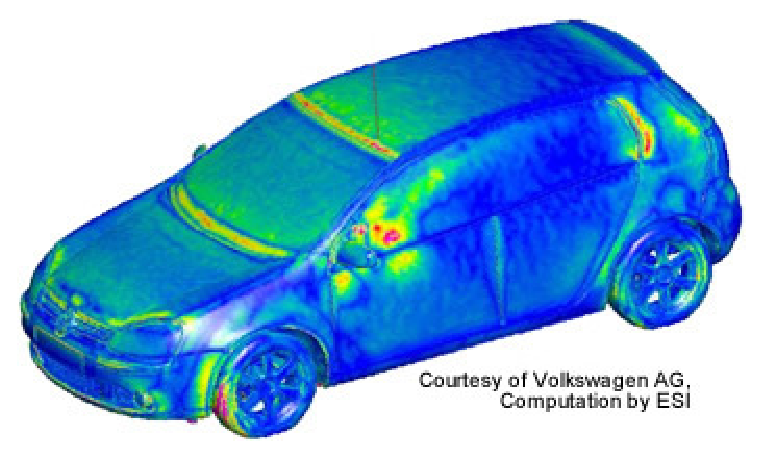
\includegraphics[width=0.3\textwidth]{./figures/adjoint_golf}}
    \hspace{1cm}
    \subfigure[Airbus: Drag]{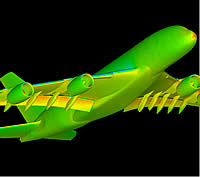
\includegraphics[width=0.3\textwidth]{./figures/airbus}}
  \end{figure}
  \begin{center}
    $
    J: \mathbb{R}^n \rightarrow \mathbb{R}, J(\mathbf{u})
    $
    $$
    \minimize_{\mathbf{u} \in \mathbb{R}^n}\;  J(\mathbf{u}) 
    $$
  \end{center}
  \begin{itemize}
    \item Geometry $\mathbf{x} \rightarrow \mathbf{u}(\mathbf{x})$: $n$ grid
      points
    \item Shape optimization: Minimize drag $J$
    \item \alert{Derivative based optimization $\rightarrow$ gradient $\nabla
      J$, input dimension $\gg$ output dimension}
  \end{itemize}
\end{frame}

\begin{frame}
  \frametitle{Motivation: Large-Scale Adjoints}
\begin{figure}
\centering
\scalebox{1}
{
  \begin{pspicture}(0,0)(9,4)
    \psframe(1,1)(3,3)
    \rput(2,3.5){\Large{Process $a$}}
  \rput(2,0.5){\Large{Send($x$,$b$)}}

  \rput(4.5,2.5){\Large{$x$}}
  \psline[arrowsize=4pt 6]{->}(3,2)(6,2)

    \psframe(6,1)(8,3)
    \rput(7,3.5){\Large{Process $b$}}
  \rput(7,0.5){\Large{Recv($x$,$a$)}}
  \end{pspicture}
}
\end{figure}
  {\bf What is different on large-scale systems?}
  \begin{itemize}
    \item Parallization: Read $\rightarrow$ write, write $\rightarrow$ read
    \item Implicit parallelism (e.g. OpenMP)
    \item Explicit parallelism (e.g. MPI)
    \item \alert{Checkpointing}
  \end{itemize}
\end{frame}

\begin{frame}
  \frametitle{Adjoint Checkpointing}
  {\bf Assumption:}
  \begin{center}
    Scalar cost function $J$ is composed of a time step based problem with time step
    function $F$.
  \end{center}

  {\bf Forward Computation:}
  $$\mathbf{u}_{t+1}=F(\mathbf{u}_t)$$
  {\bf Adjoint/Reverse Computation:}
  $$\bar{\mathbf{u}}_t=\left(\nabla F(\mathbf{u}_t)\right)^{T} \cdot
  \bar{\mathbf{u}}_{t+1}=\bar{F}(\mathbf{u}_t,\bar{\mathbf{u}}_{t+1})$$
  {\bf Example}
  $$\mathbf{u}_1=F(\mathbf{u}_0),\ \mathbf{u}_2=F(\mathbf{u}_1),\
  \mathbf{u}_3=F(\mathbf{u}_2)$$
  $$\bar{\mathbf{u}}_2=\bar{F}(\mathbf{u}_2,\bar{\mathbf{u}}_3),\
  \bar{\mathbf{u}}_1=\bar{F}(\mathbf{u}_1,\bar{\mathbf{u}}_2),\
  \bar{\mathbf{u}}_0=\bar{F}(\mathbf{u}_0,\bar{\mathbf{u}}_1)$$
\end{frame}

\begin{frame}
    \frametitle{Nek5000\footnote{\cite{nekmanual}, \url{http://nek5000.mcs.anl.gov/}}}
    \begin{itemize}
      \item Spectral Element Method (SEM) based CFD solver
      \item Solves incompressible Navier-Stokes
      \item Spectrally accurate (polynomial order of up to 20)
      \item Halo exchange has always same size independent of order
      \item Highly scalable: $10^{12}$ grid points scale up to $10^8$ processors
    \end{itemize}
\begin{figure}
  \centering
  \subfigure[Flow around fuel rods]{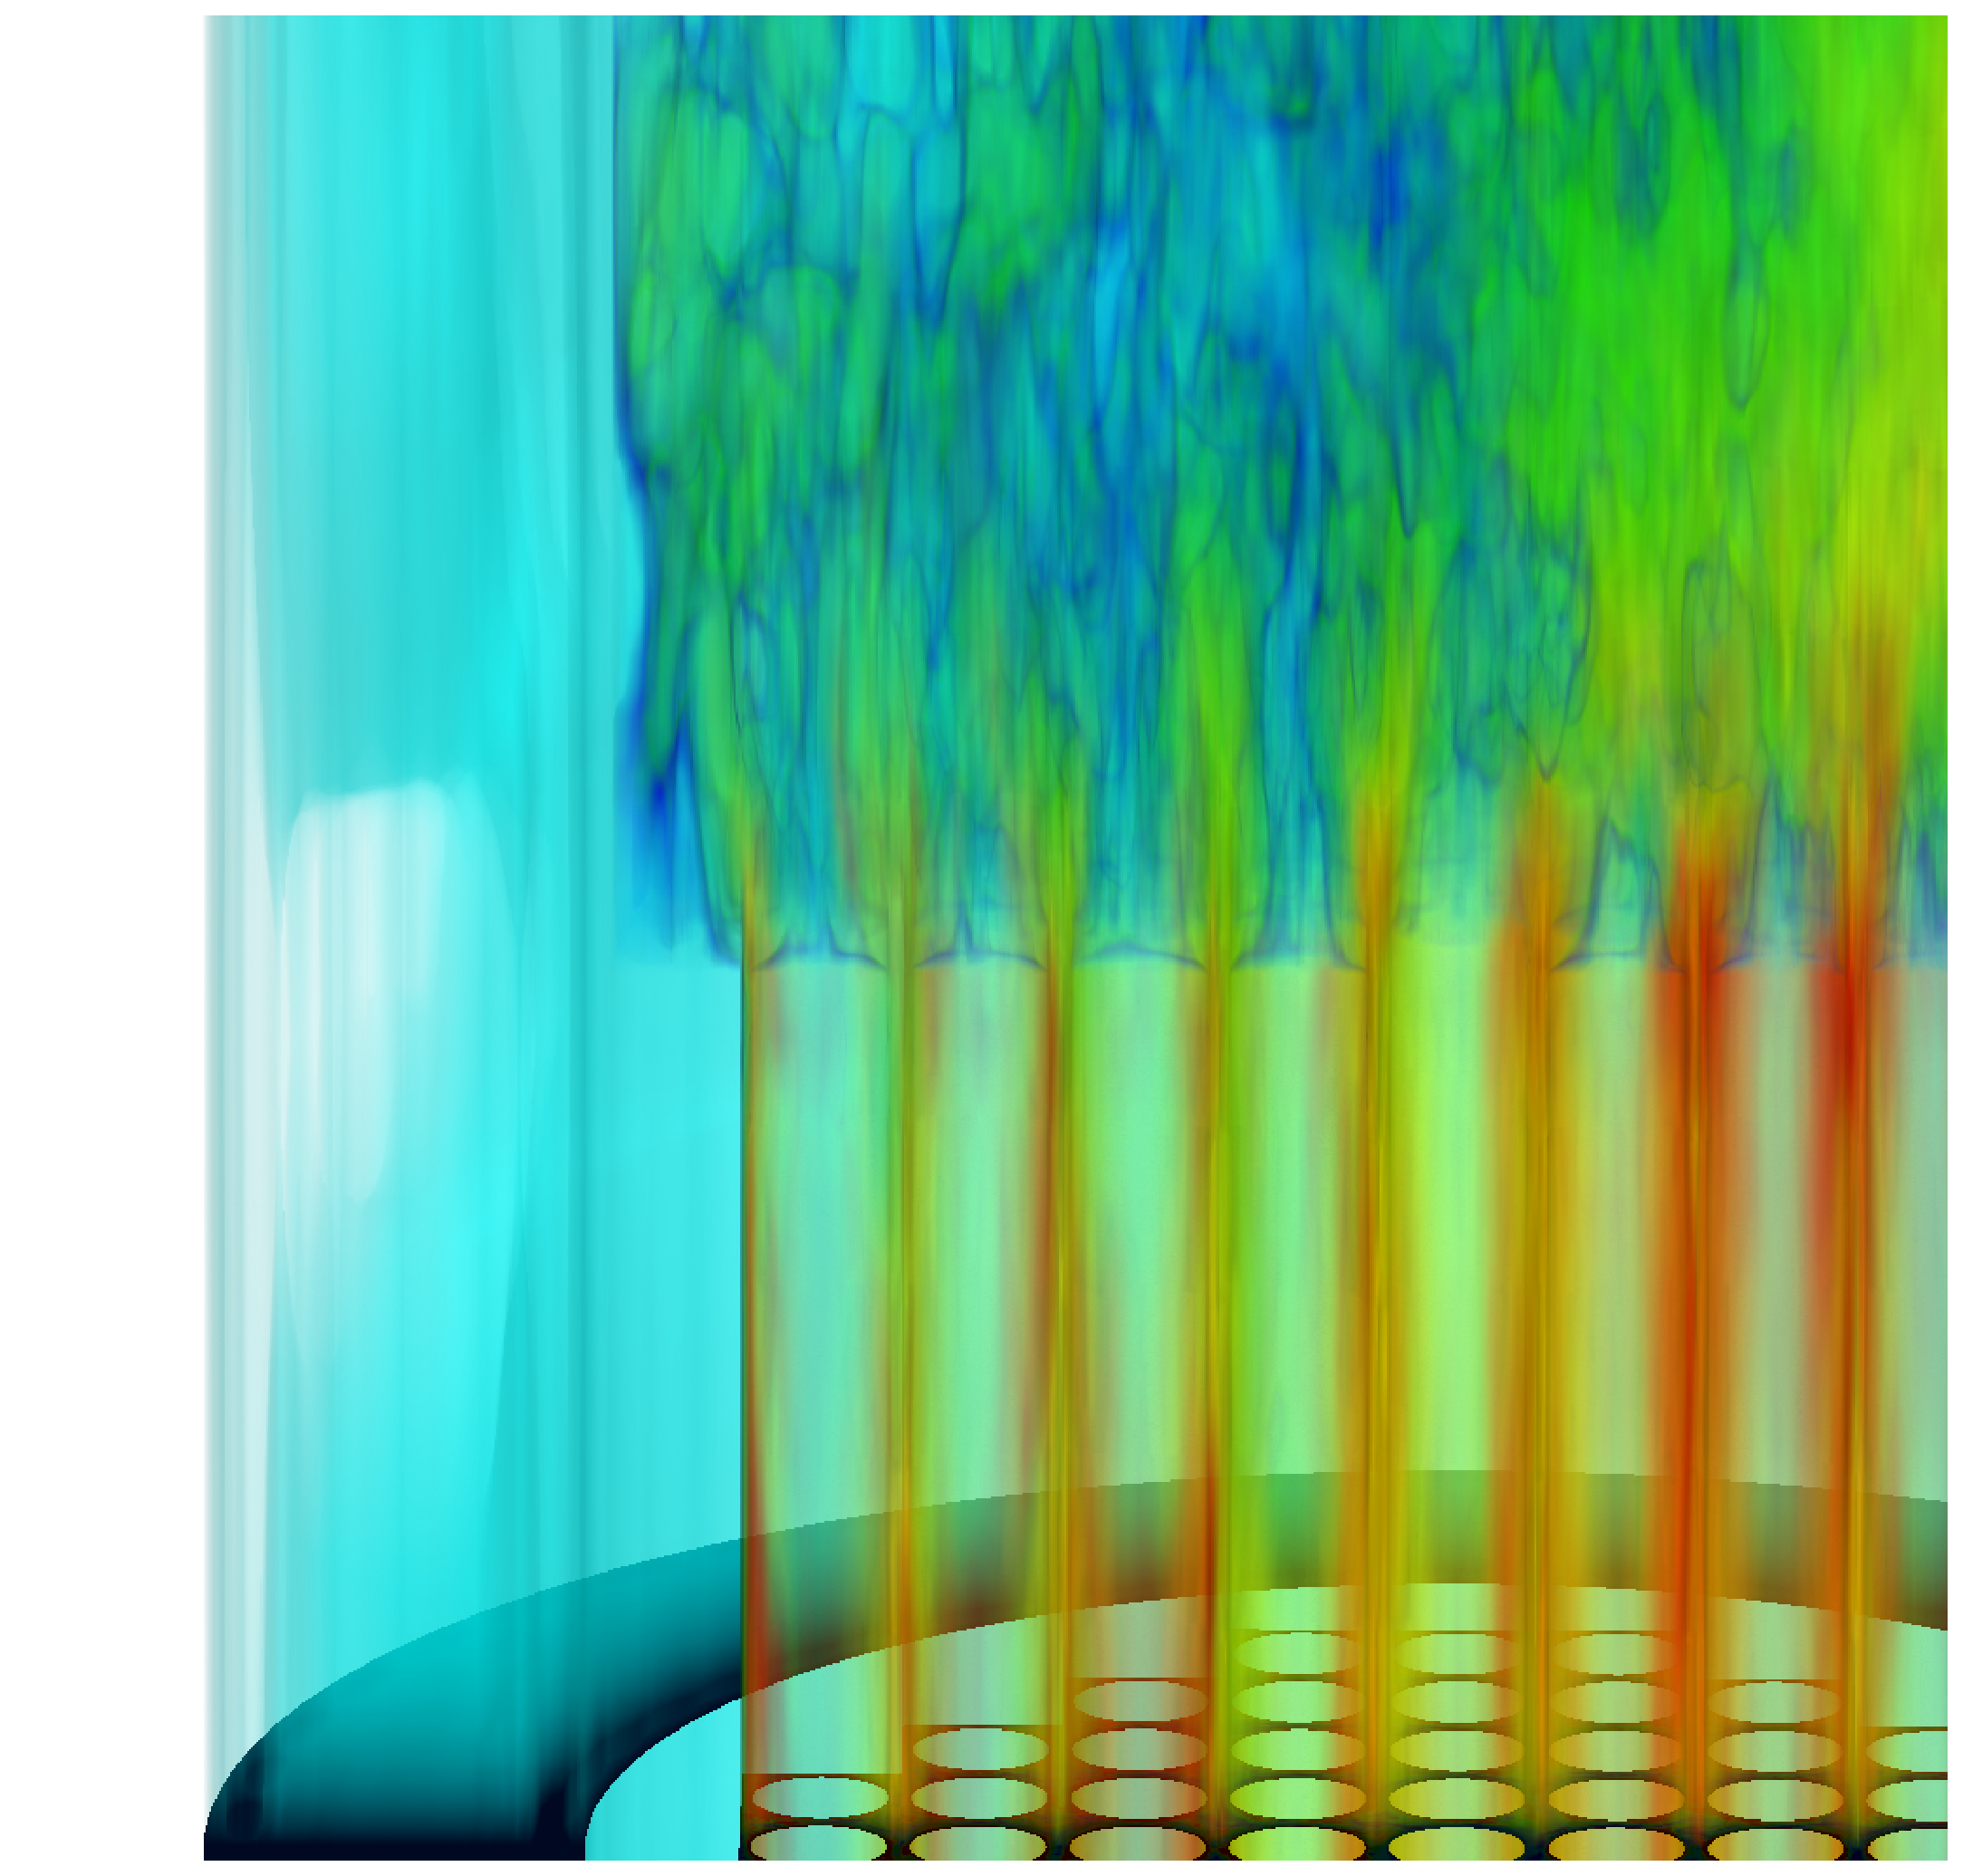
\includegraphics[width=0.45\textwidth]{./figures/nek_1}}
  \subfigure[Flow in a straight pipe at $Re=1000$]{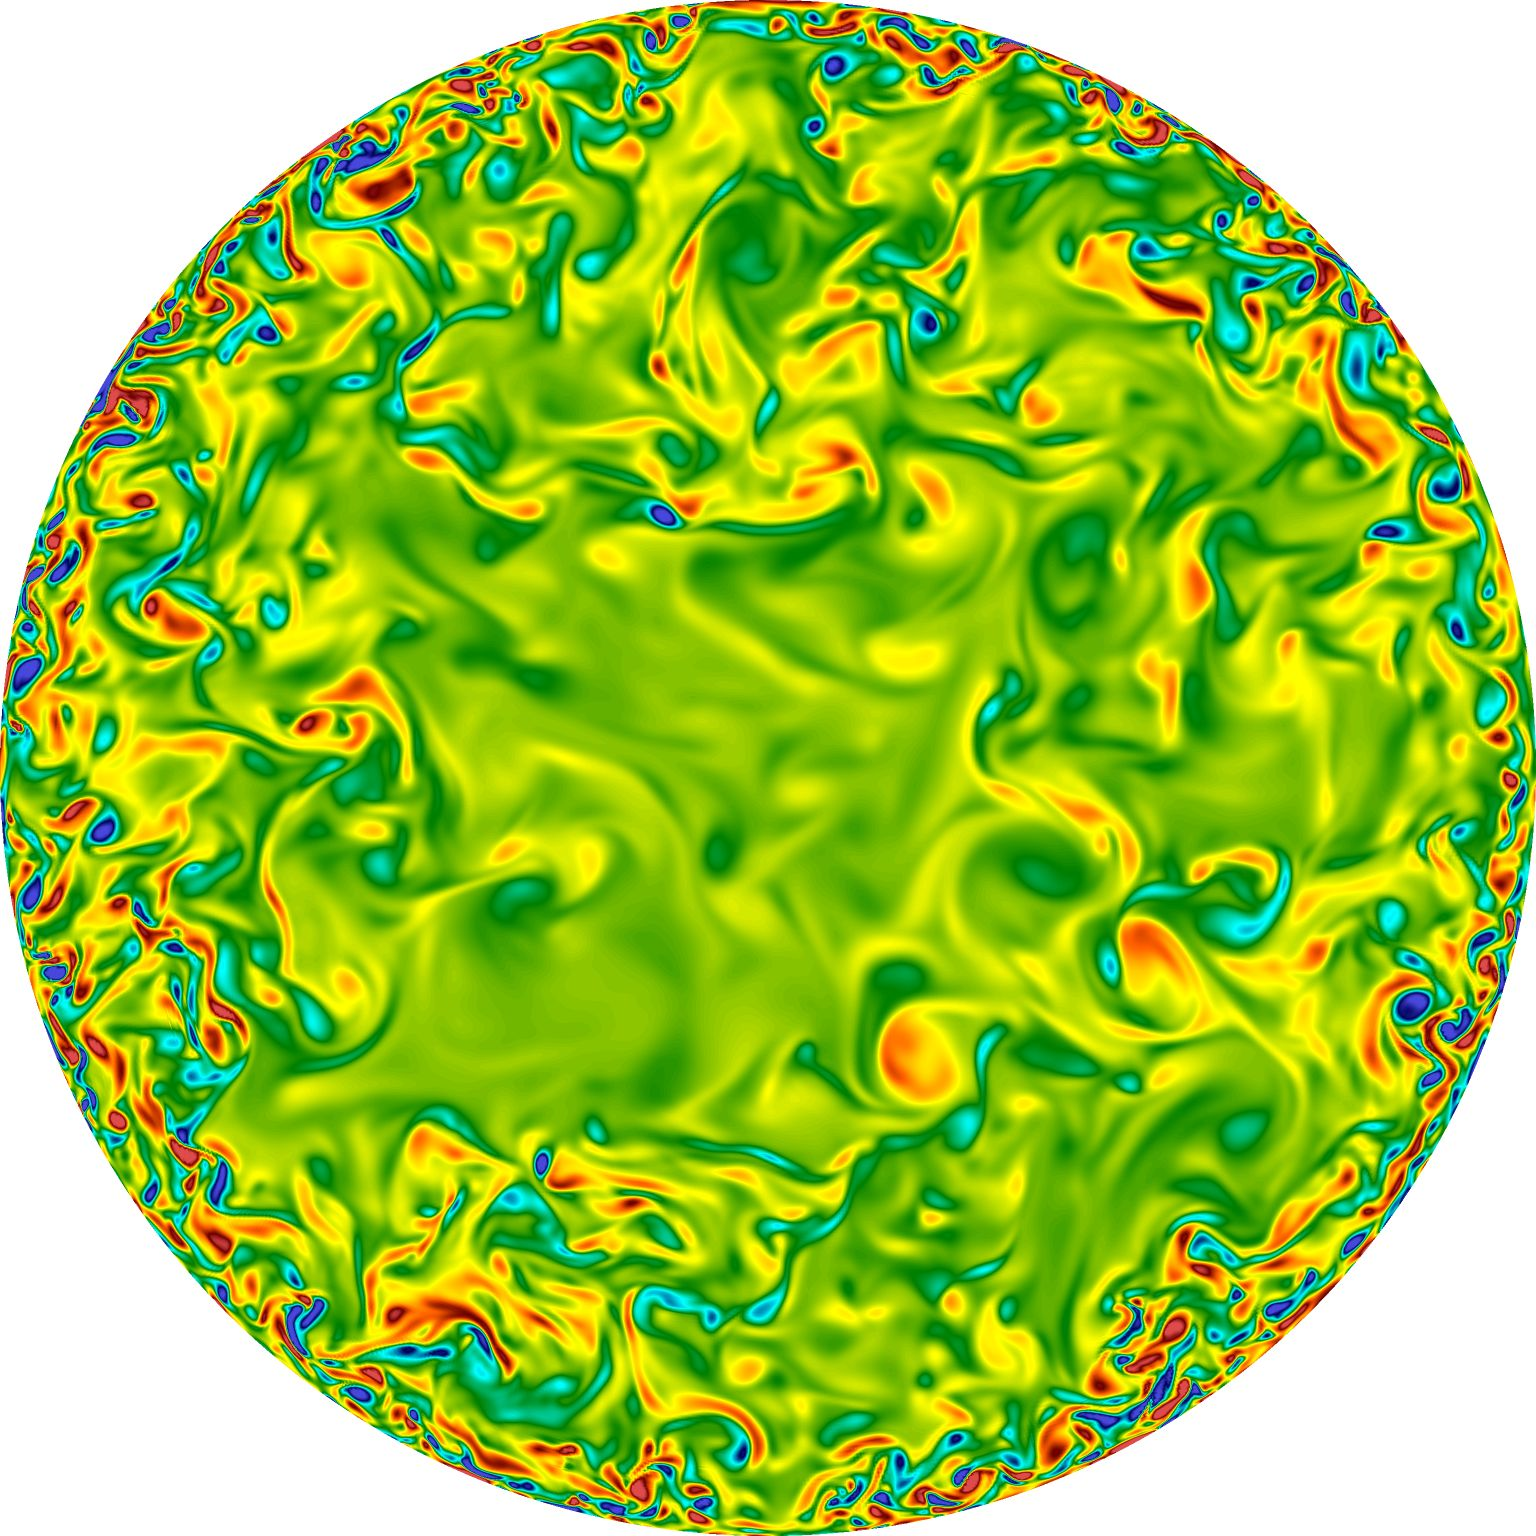
\includegraphics[width=0.45\textwidth]{./figures/nek_2}}
\end{figure}
\end{frame}



\begin{frame}{Adjoints in Nek5000}

  {\bf Nek5000}

  \begin{itemize}
    \item Development started 'in the late 80s', well validated
    \item Open-source, written in F77 and C (80000 lines, no dynamic memory)
    \item Only one model: Navier-Stokes
    \item One code, no 3rd party libraries
  \end{itemize}
  {\bf Ingredients for adjoints in Nek5000:}
  \begin{itemize}
    \item Direct numerical solver $\rightarrow$ continuous adjoint is equivalent
      to discrete adjoint
    \item Dual equations are already implemented
    \item \alert{Data flow reversal, checkpointing}
  \end{itemize}
\end{frame}


\begin{frame}[fragile]
  \frametitle{Continuous/Analytic Adjoints}
  \begin{block}{Navier-Stokes (Primal)}
    $$
    \dfrac{\partial \mathbf{u}}{\partial{t}}+(\mathbf{u} \cdot
    \nabla)\mathbf{u}-\dfrac{1}{Re} \nabla^2 \mathbf{u}+\nabla{p}=\mathbf{f}
    $$
  \end{block}
  \begin{block}{Adjoint Navier-Stokes wrt. $\mathbf{u}$ (Dual)}
    $$
    \dfrac{\partial
    \bar{\mathbf{u}}}{\partial{t}}+(\mathbf{\nabla{\alert{u}}})^{\intercal}\bar{\mathbf{u}} -
    \mathbf{\alert{u}}\cdot \nabla{\bar{\mathbf{u}}}
    +\dfrac{1}{Re} \nabla^2 \bar{\mathbf{u}}+\nabla{\bar{p}}=\mathbf{f}
    $$
  \end{block}
  \begin{itemize}
    \item Velocity field $\mathbf{u}$, pressure $p$, forcing $\mathbf{f}$ and Reynolds
      number $Re$
    \item Nonlinearity of the primal: Save velocity field $\alert{u_t}$ at every time step $t$
    \item Timesteps of the adjoint model are executed in reverse order!
    \item Use cases: flow stability, mixing, geometry optimization, data assimilation
      (more in \cite{nekcontadjoints})
  \end{itemize}
\end{frame}



\begin{frame}{Control and Data Flow Reversal}
\begin{center}
\begin{align*}
\mathbf{u}_{t+1}&=F_t(\mathbf{u}_t)\\
\bar{\mathbf{u}}_{t}&=\bar{F}_t(\mathbf{u}_t,\bar{\mathbf{u}}_{t+1})
\end{align*}
\end{center}
\begin{center}
  \begin{adjustbox}{width=\textwidth,keepaspectratio}
    \begin{pspicture}(-1,-2.5)(19,1)
      \psline[arrowsize=5pt,linecolor=red]{->}(0,1.5)(0,0.5)
      \psline[arrowsize=5pt,linecolor=red]{->}(2,1.5)(2,0.5)
      \psline[arrowsize=5pt,linecolor=red]{->}(4,1.5)(4,0.5)
      \psline[arrowsize=5pt,linecolor=red]{->}(6,1.5)(6,0.5)
      \psline[arrowsize=5pt,linecolor=red]{->}(8,1.5)(8,0.5)
      \psline[arrowsize=5pt,linecolor=red]{->}(10,1.5)(10,0.5)
      \psline[arrowsize=5pt,linecolor=red]{->}(12,1.5)(12,0.5)
      \psline[arrowsize=5pt,linecolor=red]{->}(14,1.5)(14,0.5)
      \psline[arrowsize=5pt,linecolor=red]{->}(16,1.5)(16,0.5)
      \pscircle(0,0){0.5}
      \pscircle(2,0){0.5}
      \pscircle(4,0){0.5}
      \pscircle(6,0){0.5}
      \pscircle(8,0){0.5}
      \pscircle(10,0){0.5}
      \pscircle(12,0){0.5}
      \pscircle(14,0){0.5}
      \pscircle(16,0){0.5}
      \pscircle(18,0){0.5}
      \psline[arrowsize=5pt,linecolor=red]{<-}(0,-1)(0,-2.0)
      \psline[arrowsize=5pt,linecolor=red]{<-}(2,-1)(2,-2.0)
      \psline[arrowsize=5pt,linecolor=red]{<-}(4,-1)(4,-2.0)
      \psline[arrowsize=5pt,linecolor=red]{<-}(6,-1)(6,-2.0)
      \psline[arrowsize=5pt,linecolor=red]{<-}(8,-1)(8,-2.0)
      \psline[arrowsize=5pt,linecolor=red]{<-}(10,-1)(10,-2.0)
      \psline[arrowsize=5pt,linecolor=red]{<-}(12,-1)(12,-2.0)
      \psline[arrowsize=5pt,linecolor=red]{<-}(14,-1)(14,-2.0)
      \psline[arrowsize=5pt,linecolor=red]{<-}(16,-1)(16,-2.0)
      \pscircle(0,-2.5){0.5}
      \pscircle(2,-2.5){0.5}
      \pscircle(4,-2.5){0.5}
      \pscircle(6,-2.5){0.5}
      \pscircle(8,-2.5){0.5}
      \pscircle(10,-2.5){0.5}
      \pscircle(12,-2.5){0.5}
      \pscircle(14,-2.5){0.5}
      \pscircle(16,-2.5){0.5}
      \pscircle(18,-2.5){0.5}

      \rput(0,0){0}
      \rput(2,0){1}
      \rput(4,0){2}
      \rput(6,0){3}
      \rput(8,0){4}
      \rput(10,0){5}
      \rput(12,0){6}
      \rput(14,0){7}
      \rput(16,0){8}
      \rput(18,0){9}
      \rput(0,-2.5){0}
      \rput(2,-2.5){1}
      \rput(4,-2.5){2}
      \rput(6,-2.5){3}
      \rput(8,-2.5){4}
      \rput(10,-2.5){5}
      \rput(12,-2.5){6}
      \rput(14,-2.5){7}
      \rput(16,-2.5){8}
      \rput(18,-2.5){9}

      \psline[arrowsize=5pt]{->}(0.5,0)(1.5,0)
      \psline[arrowsize=5pt]{->}(2.5,0)(3.5,0)
      \psline[arrowsize=5pt]{->}(4.5,0)(5.5,0)
      \psline[arrowsize=5pt]{->}(6.5,0)(7.5,0)
      \psline[arrowsize=5pt]{->}(8.5,0)(9.5,0)
      \psline[arrowsize=5pt]{->}(10.5,0)(11.5,0)
      \psline[arrowsize=5pt]{->}(12.5,0)(13.5,0)
      \psline[arrowsize=5pt]{->}(14.5,0)(15.5,0)
      \psline[arrowsize=5pt]{->}(16.5,0)(17.5,0)
      \psline[arrowsize=5pt]{<-}(0.5,-2.5)(1.5,-2.5)
      \psline[arrowsize=5pt]{<-}(2.5,-2.5)(3.5,-2.5)
      \psline[arrowsize=5pt]{<-}(4.5,-2.5)(5.5,-2.5)
      \psline[arrowsize=5pt]{<-}(6.5,-2.5)(7.5,-2.5)
      \psline[arrowsize=5pt]{<-}(8.5,-2.5)(9.5,-2.5)
      \psline[arrowsize=5pt]{<-}(10.5,-2.5)(11.5,-2.5)
      \psline[arrowsize=5pt]{<-}(12.5,-2.5)(13.5,-2.5)
      \psline[arrowsize=5pt]{<-}(14.5,-2.5)(15.5,-2.5)
      \psline[arrowsize=5pt]{<-}(16.5,-2.5)(17.5,-2.5)
      \psline[arrowsize=5pt]{->}(18,-0.5)(18,-2.0)
    \end{pspicture}
  \end{adjustbox}
\end{center}
\begin{itemize}
  \item Most of checkpointing research in Algorithmic/Automatic Differentiation
    (AD)
  \item Nek: $\approx$ 100GB/checkpoint, 100000 timesteps, 1 timestep/s
  \item \alert{10 PB} of checkpoints
  \item Required bandwith: $100\cdot8$/s=\alert{800Gbit/s}
\end{itemize}
\end{frame}

\begin{frame}{Nonlinear Adjoint Models in Practice}
  \begin{itemize}
    \item {\color{blue}Interpolation} of checkpoints
\begin{figure}[h]
  \begin{adjustbox}{width=\textwidth,keepaspectratio}
    \begin{pspicture}(-1,-2.5)(19,1)
      \psline[arrowsize=5pt,linecolor=red]{->}(0,1.5)(0,0.5)
      \psline[arrowsize=5pt,linecolor=red]{->}(8,1.5)(8,0.5)
      \psline[arrowsize=5pt,linecolor=red]{->}(16,1.5)(16,0.5)
      \pscircle(0,0){0.5}
      \pscircle(2,0){0.5}
      \pscircle(4,0){0.5}
      \pscircle(6,0){0.5}
      \pscircle(8,0){0.5}
      \pscircle(10,0){0.5}
      \pscircle(12,0){0.5}
      \pscircle(14,0){0.5}
      \pscircle(16,0){0.5}
      \pscircle(18,0){0.5}
      \psline[arrowsize=5pt,linecolor=red]{<-}(0,-1)(0,-2.0)
      \psline[linestyle=dashed,arrowsize=5pt,linecolor=blue]{<-}(2,-1)(2,-2.0)
      \psline[linestyle=dashed,arrowsize=5pt,linecolor=blue]{<-}(4,-1)(4,-2.0)
      \psline[linestyle=dashed,arrowsize=5pt,linecolor=blue]{<-}(6,-1)(6,-2.0)
      \psline[arrowsize=5pt,linecolor=red]{<-}(8,-1)(8,-2.0)
      \psline[linestyle=dashed,arrowsize=5pt,linecolor=blue]{<-}(10,-1)(10,-2.0)
      \psline[linestyle=dashed,arrowsize=5pt,linecolor=blue]{<-}(12,-1)(12,-2.0)
      \psline[linestyle=dashed,arrowsize=5pt,linecolor=blue]{<-}(14,-1)(14,-2.0)
      \psline[arrowsize=5pt,linecolor=red]{<-}(16,-1)(16,-2.0)
      \pscircle(0,-2.5){0.5}
      \pscircle(2,-2.5){0.5}
      \pscircle(4,-2.5){0.5}
      \pscircle(6,-2.5){0.5}
      \pscircle(8,-2.5){0.5}
      \pscircle(10,-2.5){0.5}
      \pscircle(12,-2.5){0.5}
      \pscircle(14,-2.5){0.5}
      \pscircle(16,-2.5){0.5}
      \pscircle(18,-2.5){0.5}

      \rput(0,0){0}
      \rput(2,0){1}
      \rput(4,0){2}
      \rput(6,0){3}
      \rput(8,0){4}
      \rput(10,0){5}
      \rput(12,0){6}
      \rput(14,0){7}
      \rput(16,0){8}
      \rput(18,0){9}
      \rput(0,-2.5){0}
      \rput(2,-2.5){1}
      \rput(4,-2.5){2}
      \rput(6,-2.5){3}
      \rput(8,-2.5){4}
      \rput(10,-2.5){5}
      \rput(12,-2.5){6}
      \rput(14,-2.5){7}
      \rput(16,-2.5){8}
      \rput(18,-2.5){9}

      \psline[arrowsize=5pt]{->}(0.5,0)(1.5,0)
      \psline[arrowsize=5pt]{->}(2.5,0)(3.5,0)
      \psline[arrowsize=5pt]{->}(4.5,0)(5.5,0)
      \psline[arrowsize=5pt]{->}(6.5,0)(7.5,0)
      \psline[arrowsize=5pt]{->}(8.5,0)(9.5,0)
      \psline[arrowsize=5pt]{->}(10.5,0)(11.5,0)
      \psline[arrowsize=5pt]{->}(12.5,0)(13.5,0)
      \psline[arrowsize=5pt]{->}(14.5,0)(15.5,0)
      \psline[arrowsize=5pt]{->}(16.5,0)(17.5,0)
      \psline[arrowsize=5pt]{<-}(0.5,-2.5)(1.5,-2.5)
      \psline[arrowsize=5pt]{<-}(2.5,-2.5)(3.5,-2.5)
      \psline[arrowsize=5pt]{<-}(4.5,-2.5)(5.5,-2.5)
      \psline[arrowsize=5pt]{<-}(6.5,-2.5)(7.5,-2.5)
      \psline[arrowsize=5pt]{<-}(8.5,-2.5)(9.5,-2.5)
      \psline[arrowsize=5pt]{<-}(10.5,-2.5)(11.5,-2.5)
      \psline[arrowsize=5pt]{<-}(12.5,-2.5)(13.5,-2.5)
      \psline[arrowsize=5pt]{<-}(14.5,-2.5)(15.5,-2.5)
      \psline[arrowsize=5pt]{<-}(16.5,-2.5)(17.5,-2.5)
      \psline[arrowsize=5pt]{->}(18,-0.5)(18,-2.0)
    \end{pspicture}
  \end{adjustbox}
\end{figure}
    \item Linearization, \citet*{peplinski2014stability} 
\begin{center}
\begin{align*}
\mathbf{u}_{t+1}&=F_t(\mathbf{u}_t)\\
\bar{\mathbf{u}}_{t}&=\bar{F}_t(\mathbf{u_B},\bar{\mathbf{u}}_{t+1})
\end{align*}
\end{center}
    \item We want no approximation  
    \item Full nonlinear adjoint considered as too hard or no use case
  \end{itemize}
\end{frame}

\begin{frame}{Data Flow Reversal}
\begin{center}
  {\bf Trade-off: Checkpoint memory vs. recomputation}
\end{center}
\begin{figure}[h]
  \begin{adjustbox}{width=\textwidth,keepaspectratio}
    \begin{pspicture}(-1,-1)(19,1)
      \psline[arrowsize=5pt,linecolor=red]{->}(0,1.5)(0,0.5)
      \pscircle(0,0){0.5}
      \pscircle(2,0){0.5}
      \pscircle(4,0){0.5}
      \pscircle(6,0){0.5}
      \pscircle(8,0){0.5}
      \pscircle(10,0){0.5}
      \pscircle(12,0){0.5}
      \pscircle(14,0){0.5}
      \psline[arrowsize=5pt,linecolor=red]{<->}(16,1.5)(16,0.5)
      \pscircle(16,0){0.5}
      \pscircle(18,0){0.5}

      \rput(0,0){0}
      \rput(2,0){1}
      \rput(4,0){2}
      \rput(6,0){3}
      \rput(8,0){4}
      \rput(10,0){5}
      \rput(12,0){6}
      \rput(14,0){7}
      \rput(16,0){8}
      \rput(18,0){9}

      \psline[arrowsize=5pt]{->}(0.5,0)(1.5,0)
      \psline[arrowsize=5pt]{->}(2.5,0)(3.5,0)
      \psline[arrowsize=5pt]{->}(4.5,0)(5.5,0)
      \psline[arrowsize=5pt]{->}(6.5,0)(7.5,0)
      \psline[arrowsize=5pt]{->}(8.5,0)(9.5,0)
      \psline[arrowsize=5pt]{->}(10.5,0)(11.5,0)
      \psline[arrowsize=5pt]{->}(12.5,0)(13.5,0)
      \psline[arrowsize=5pt]{->}(14.5,0)(15.5,0)
      \psline[arrowsize=5pt,linearc=.25]{->}(16.5,0)(17,1)(17.5,0)
      \psline[arrowsize=5pt,linearc=.25]{<-}(16.5,0)(17,-1)(17.5,0)
    \end{pspicture}
  \end{adjustbox}
  \begin{adjustbox}{width=\textwidth,keepaspectratio}
    \begin{pspicture}(-1,-1)(19,1)
      \psline[arrowsize=5pt,linecolor=red]{<-}(0,1.5)(0,0.5)
      \pscircle(0,0){0.5}
      \pscircle(2,0){0.5}
      \pscircle(4,0){0.5}
      \pscircle(6,0){0.5}
      \pscircle(8,0){0.5}
      \pscircle(10,0){0.5}
      \pscircle(12,0){0.5}
      \psline[arrowsize=5pt,linecolor=red]{<->}(14,1.5)(14,0.5)
      \pscircle(14,0){0.5}
      \pscircle(16,0){0.5}

      \rput(0,0){0}
      \rput(2,0){1}
      \rput(4,0){2}
      \rput(6,0){3}
      \rput(8,0){4}
      \rput(10,0){5}
      \rput(12,0){6}
      \rput(14,0){7}
      \rput(16,0){8}
      \rput(-0.5,0){\color{white} .}
      \rput(18.5,0){\color{white} .}

      \psline[arrowsize=5pt]{->}(0.5,0)(1.5,0)
      \psline[arrowsize=5pt]{->}(2.5,0)(3.5,0)
      \psline[arrowsize=5pt]{->}(4.5,0)(5.5,0)
      \psline[arrowsize=5pt]{->}(6.5,0)(7.5,0)
      \psline[arrowsize=5pt]{->}(8.5,0)(9.5,0)
      \psline[arrowsize=5pt]{->}(10.5,0)(11.5,0)
      \psline[arrowsize=5pt]{->}(12.5,0)(13.5,0)
      \psline[arrowsize=5pt,linearc=.25]{->}(14.5,0)(15,1)(15.5,0)
      \psline[arrowsize=5pt,linearc=.25]{<-}(14.5,0)(15,-1)(15.5,0)
    \end{pspicture}
  \end{adjustbox}
  \begin{adjustbox}{width=\textwidth,keepaspectratio}
    \begin{pspicture}(-1,-1)(19,1)
      \rput(9,0){\Huge ...}
      \rput(-0.5,0){\color{white} .}
      \rput(18.5,0){\color{white} .}
    \end{pspicture}
  \end{adjustbox}
  \begin{adjustbox}{width=\textwidth,keepaspectratio}
    \begin{pspicture}(-1,-1)(19,1)
      \psline[arrowsize=5pt,linecolor=red]{<-}(0,1.5)(0,0.5)
      \pscircle(0,0){0.5}
      \pscircle(2,0){0.5}

      \rput(0,0){0}
      \rput(2,0){1}
      \rput(-0.5,0){\color{white} .}
      \rput(18.5,0){\color{white} .}

      \psline[arrowsize=5pt,linearc=.25]{->}(0.5,0)(1,1)(1.5,0)
      \psline[arrowsize=5pt,linearc=.25]{<-}(0.5,0)(1,-1)(1.5,0)
    \end{pspicture}
  \end{adjustbox}
\end{figure}
\begin{itemize}
  \item For $t=10$ sub-steps $9+8+\ldots+1=\frac{t^2}{2}$ recomputations are needed
  \item Only two checkpoint (inputs)
\end{itemize}
\end{frame}

\begin{frame}[fragile]
  \frametitle{Hardware and Software Assumptions}
  \begin{center}
    {\Large \bf Assumptions for two-level checkpointing }
  \end{center}
  \begin{itemize}
    \item {\bf A1} The total number of time steps is a priori unknown
    \item {\bf A2} Disk I/O is limited only by bandwidth and latency (not by size)
    \item {\bf A3} There may be infinite disk checkpoints
    \item {\bf A4} Memory is bound by size
    \item {\bf A5} Memory bandwidth is infinite (storing/restoring is 0 cost compared to
      the rest of the application)
  \end{itemize}
  \begin{itemize}
    \item Disk I/O is asynchronous (synchronous checkpointing presented in
      \cite{hovlandtwolevel})
  \end{itemize}
\end{frame}

\begin{frame}
  \frametitle{Assumptions applied to Mira}
  \begin{figure}
    \begin{adjustbox}{width=0.8\textwidth,keepaspectratio}
      \begin{pspicture}(0,-1.15)(11,2)
        \rput[bl](0.15,1.6){Mira}
        \psframe(0,-1.15)(2,2)
        \psframe(0.15,-1)(1.15,1.5)
        \psframe(1.30,-1)(1.85,1.5)
        \rput{90}(0.65,0.25){Compute Nodes}
        \rput{90}(1.575,0.25){I/O Nodes}
        \psline[arrowsize=5pt]{->}(2,0.425)(6,0.425)
        \rput(4,1){Storage Area Network}
        \rput(4,-0.15){$\gg$ 2GB/s}
        \psframe(6,-1.15)(7,2)
        \rput{90}(6.5,0.25){Disks}
        \psline[arrowsize=5pt]{->}(7,0.425)(10,0.425)
        \rput(8.5,1){Fiber}
        \psframe(10,-1.15)(11,2)
        \rput(8.5,-0.15){$\approx$ 2GB/s}
        \rput{90}(10.5,0.25){HPSS (archive)}

      \end{pspicture}
    \end{adjustbox}
    %\caption{Mira storage hierarchy. The archive is referred to as
    %{\it disk} in our algorithm. The disks on Mira are transparent and serve only
    %as a buffer between archive and Mira.}
    \label{fig:mira_setup}
  \end{figure}
  \begin{itemize}
    \item Asynchronous I/O on HPSS
    \item Only synchronous I/O on disks (per checkpoint $\approx 1 ts \approx
      1.5s$)
    \item Disks will only serve as buffer. I/O time is negligible
  \end{itemize}
\end{frame}


\begin{frame}
  \frametitle{Algorithm in a Nutshell}
  \begin{itemize}
    \item Number of disk checkpoints unlimited, memory checkpoints limited
    \item Stride q for disk checkpoints is determined by disk bandwidth (store
      as many as possible) during the forward run\\
  \begin{adjustbox}{width=\textwidth,keepaspectratio}
    \begin{pspicture}(-1,-0.5)(31,2.5)
      \pscircle(0,0){0.5}
      \pscircle(2,0){0.5}
      \pscircle(4,0){0.5}
      \pscircle(6,0){0.5}
      \pscircle(8,0){0.5}
      \pscircle(10,0){0.5}
      \pscircle(12,0){0.5}
      \pscircle(14,0){0.5}
      \pscircle(16,0){0.5}
      \pscircle(18,0){0.5}
      \pscircle(20,0){0.5}
      \pscircle(22,0){0.5}
      \pscircle(24,0){0.5}
      \pscircle(26,0){0.5}
      \pscircle(28,0){0.5}

      \psline[arrowsize=5pt,linecolor=red]{->}(0,1.5)(0,0.5)
      \rput(0,0){0}
      \rput(2,0){1}
      \rput(4,0){2}
      \rput(6,0){3}
      \psline[arrowsize=5pt,linecolor=red]{->}(8,1.5)(8,0.5)
      \rput(8,0){4}
      \rput(10,0){5}
      \rput(12,0){6}
      \psline[arrowsize=5pt,linecolor=red]{->}(14,1.5)(14,0.5)
      \rput(14,0){7}
      \rput(16,0){8}
      \rput(18,0){9}
      \rput(20,0){10}
      \rput(22,0){11}
      \psline[arrowsize=5pt,linecolor=red]{->}(24,1.5)(24,0.5)
      \rput(24,0){12}
      \rput(26,0){13}
      \rput(28,0){14}

      \psline[arrowsize=5pt]{->}(0.5,0)(1.5,0)
      \psline[arrowsize=5pt]{->}(2.5,0)(3.5,0)
      \psline[arrowsize=5pt]{->}(4.5,0)(5.5,0)
      \psline[arrowsize=5pt]{->}(6.5,0)(7.5,0)
      \psline[arrowsize=5pt]{->}(8.5,0)(9.5,0)
      \psline[arrowsize=5pt]{->}(10.5,0)(11.5,0)
      \psline[arrowsize=5pt]{->}(12.5,0)(13.5,0)
      \psline[arrowsize=5pt]{->}(14.5,0)(15.5,0)
      \psline[arrowsize=5pt]{->}(16.5,0)(17.5,0)
      \psline[arrowsize=5pt]{->}(18.5,0)(19.5,0)
      \psline[arrowsize=5pt]{->}(20.5,0)(21.5,0)
      \psline[arrowsize=5pt]{->}(22.5,0)(23.5,0)
      \psline[arrowsize=5pt]{->}(24.5,0)(25.5,0)
      \psline[arrowsize=5pt,linearc=.25]{->}(26.5,0)(27,1)(27.5,0)
      \psline[arrowsize=5pt,linearc=.25]{<-}(26.5,0)(27,-1)(27.5,0)

      \psline[arrowsize=5pt,linecolor=red]{<->}(0.5,1)(7.5,1)
      \rput(4,2){\Huge{\color{red}{$q$}}}
    \end{pspicture}
  \end{adjustbox}
\item Memory checkpointing on each stride of length q using revolve algorithm
  \cite{revolve} in
  the adjoint run.\\
  \begin{adjustbox}{width=\textwidth,keepaspectratio}
    \begin{pspicture}(-0.5,-1)(14.5,2)
      \pscircle(0,0){0.5}
      \pscircle(2,0){0.5}
      \pscircle(4,0){0.5}
      \pscircle(6,0){0.5}
      \pscircle(8,0){0.5}
      \pscircle(10,0){0.5}
      \pscircle(12,0){0.5}
      \pscircle(14,0){0.5}

      \psline[arrowsize=5pt,linecolor=red]{<-}(0,1.5)(0,0.5)
      \rput(0,0){0}
      \rput(2,0){1}
      \rput(4,0){2}
      \psline[linestyle=dashed,arrowsize=5pt,linecolor=blue]{->}(6,1.5)(6,0.5)
      \rput(6,0){3}
      \rput(8,0){4}
      \psline[linestyle=dashed,arrowsize=5pt,linecolor=blue]{->}(10,1.5)(10,0.5)
      \rput(10,0){5}
      \rput(12,0){6}
      \rput(14,0){7}
      \rput(-0.5,0){\color{white} .}
      \rput(15.5,0){\color{white} .}

      \psline[arrowsize=5pt]{->}(0.5,0)(1.5,0)
      \psline[arrowsize=5pt]{->}(2.5,0)(3.5,0)
      \psline[arrowsize=5pt]{->}(4.5,0)(5.5,0)
      \psline[arrowsize=5pt]{->}(6.5,0)(7.5,0)
      \psline[arrowsize=5pt]{->}(8.5,0)(9.5,0)
      \psline[arrowsize=5pt]{->}(10.5,0)(11.5,0)
      \psline[arrowsize=5pt,linearc=.25]{->}(12.5,0)(13,1)(13.5,0)
      \psline[arrowsize=5pt,linearc=.25]{<-}(12.5,0)(13,-1)(13.5,0)
    \end{pspicture}

    \begin{pspicture}(8,-1)(15.5,1.5)
      \pscircle(10,0){0.5}
      \pscircle(12,0){0.5}

      \psline[linestyle=dashed,arrowsize=5pt,linecolor=blue]{<-}(10,1.5)(10,0.5)
      \rput(10,0){5}
      \rput(12,0){6}
      \rput(8,0){\color{white} .}
      \rput(18.5,0){\color{white} .}

      %\psline[arrowsize=5pt,linearc=.25]{->}(10.5,0)(11,1)(11.5,0)
      %\psline[arrowsize=5pt,linearc=.25]{<-}(10.5,0)(11,-1)(11.5,0)
      \psline[arrowsize=5pt]{<-}(10.5,0)(11.5,0)
    \end{pspicture}
  \end{adjustbox}
%\end{center}
%\begin{center}
  \begin{adjustbox}{width=0.7\textwidth,keepaspectratio}
    \begin{pspicture}(5.5,-1)(11.5,1.5)
      \pscircle(6,0){0.5}
      \pscircle(8,0){0.5}
      \pscircle(10,0){0.5}

      \psline[linestyle=dashed,arrowsize=5pt,linecolor=blue]{<-}(6,1.5)(6,0.5)
      \rput(6,0){3}
      \rput(8,0){4}
      \rput(10,0){5}
      \rput(5,0){\color{white} .}
      \rput(11.5,0){\color{white} .}

      \psline[arrowsize=5pt]{->}(6.5,0)(7.5,0)
      %\psline[arrowsize=5pt,linearc=.25]{->}(8.5,0)(9,1)(9.5,0)
      %\psline[arrowsize=5pt,linearc=.25]{<-}(8.5,0)(9,-1)(9.5,0)
      \psline[arrowsize=5pt]{<-}(8.5,0)(9.5,0)
    \end{pspicture}

    \begin{pspicture}(5,-1)(14,1.5)
      \pscircle(6,0){0.5}
      \pscircle(8,0){0.5}

      \psline[linestyle=dashed,arrowsize=5pt,linecolor=blue]{<-}(6,1.5)(6,0.5)
      \rput(6,0){3}
      \rput(8,0){4}
      \rput(5,0){\color{white} .}
      \rput(14,0){\color{white} .}

      %\psline[arrowsize=5pt,linearc=.25]{->}(6.5,0)(7,1)(7.5,0)
      %\psline[arrowsize=5pt,linearc=.25]{<-}(6.5,0)(7,-1)(7.5,0)
      \psline[arrowsize=5pt]{<-}(6.5,0)(7.5,0)
    \end{pspicture}
  \end{adjustbox}
%\end{center}
%\begin{center}
  \begin{adjustbox}{width=0.8\textwidth,keepaspectratio}
    \begin{pspicture}(-0.5,-1)(7.5,1.5)
      \pscircle(0,0){0.5}
      \pscircle(2,0){0.5}
      \pscircle(4,0){0.5}
      \pscircle(6,0){0.5}

      \psline[arrowsize=5pt,linecolor=red]{<-}(0,1.5)(0,0.5)
      \rput(0,0){0}
      \psline[linestyle=dashed,arrowsize=5pt,linecolor=blue]{->}(2,1.5)(2,0.5)
      \rput(2,0){1}
      \rput(4,0){2}
      \rput(6,0){3}
      \rput(-0.5,0){\color{white} .}
      \rput(7.5,0){\color{white} .}

      \psline[arrowsize=5pt]{->}(0.5,0)(1.5,0)
      \psline[arrowsize=5pt]{->}(2.5,0)(3.5,0)
      %\psline[arrowsize=5pt,linearc=.25]{->}(4.5,0)(5,1)(5.5,0)
      %\psline[arrowsize=5pt,linearc=.25]{<-}(4.5,0)(5,-1)(5.5,0)
      \psline[arrowsize=5pt]{<-}(4.5,0)(5.5,0)
    \end{pspicture}
    \begin{pspicture}(1,-1)(5.5,1.5)
      \pscircle(2,0){0.5}
      \pscircle(4,0){0.5}

      \psline[linestyle=dashed,arrowsize=5pt,linecolor=blue]{<-}(2,1.5)(2,0.5)
      \rput(2,0){1}
      \rput(4,0){2}
      \rput(1,0){\color{white} .}
      \rput(5.5,0){\color{white} .}

      %\psline[arrowsize=5pt,linearc=.25]{->}(2.5,0)(3,1)(3.5,0)
      %\psline[arrowsize=5pt,linearc=.25]{<-}(2.5,0)(3,-1)(3.5,0)
      \psline[arrowsize=5pt]{<-}(2.5,0)(3.5,0)
    \end{pspicture}
    \begin{pspicture}(1,-1)(5,1.5)
      \pscircle(2,0){0.5}
      \pscircle(4,0){0.5}

      \psline[arrowsize=5pt,linecolor=red]{<-}(2,1.5)(2,0.5)
      \rput(2,0){0}
      \rput(4,0){1}
      \rput(1,0){\color{white} .}
      \rput(5,0){\color{white} .}

      %\psline[arrowsize=5pt,linearc=.25]{->}(2.5,0)(3,1)(3.5,0)
      %\psline[arrowsize=5pt,linearc=.25]{<-}(2.5,0)(3,-1)(3.5,0)
      \psline[arrowsize=5pt]{<-}(2.5,0)(3.5,0)
    \end{pspicture}
  \end{adjustbox}
  \end{itemize}
\end{frame}

\begin{frame}

  \frametitle{Use Case: Lid Driven Cavity}
\begin{figure}
  \centering
  \subfigure[Primal]{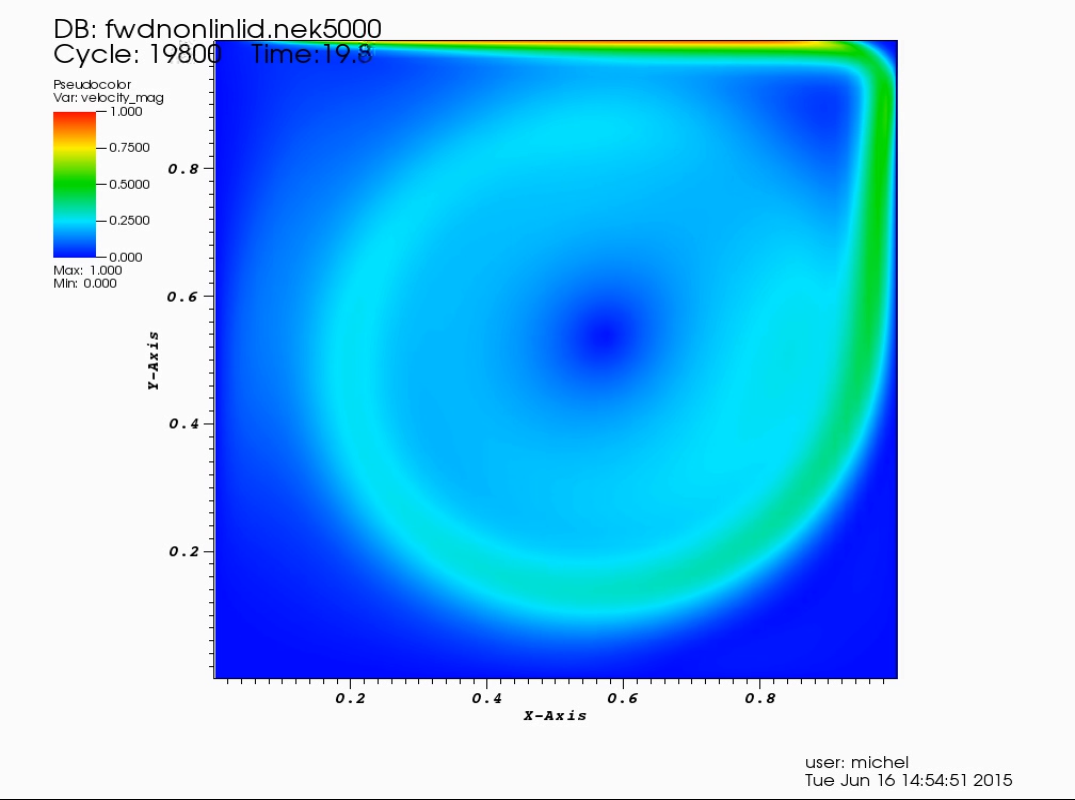
\includegraphics[width=0.45\textwidth]{./figures/primal}}
  \subfigure[Adjoint]{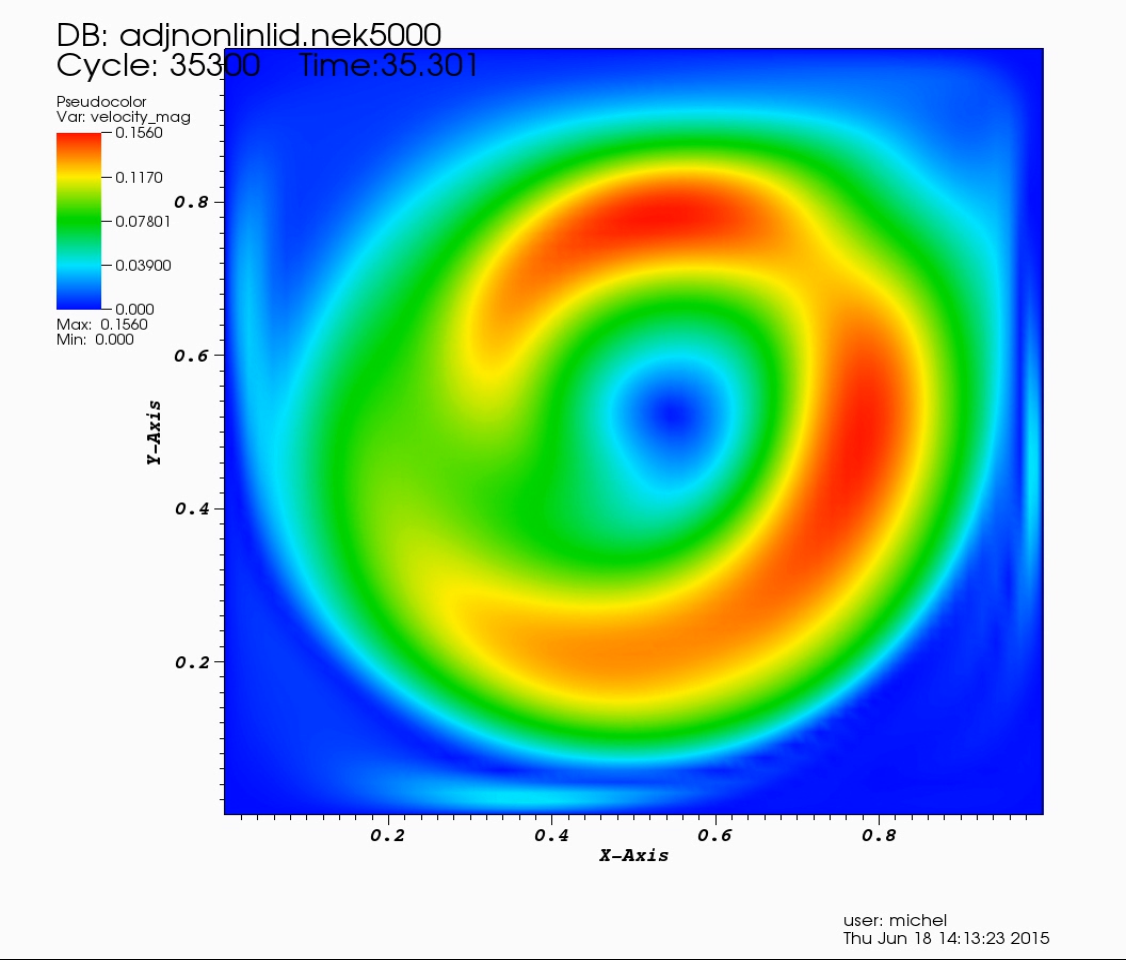
\includegraphics[width=0.45\textwidth]{./figures/dual}}
  \label{fig:fd}
\end{figure}
  \begin{itemize}
    \item Flexible use case that allows weak scaling 
    \item Kinetic energy $E_k$ at final timestep $T$: $E_k=\frac{1}{2}<\mathbf{u}_T,
      \mathbf{u}_T>$ with respect to inital
      condition $\mathbf{u}_0$
  \end{itemize}
\end{frame}

\begin{frame}
  \frametitle{Validation}
\begin{figure}
  \centering
  \subfigure[Adjoint]{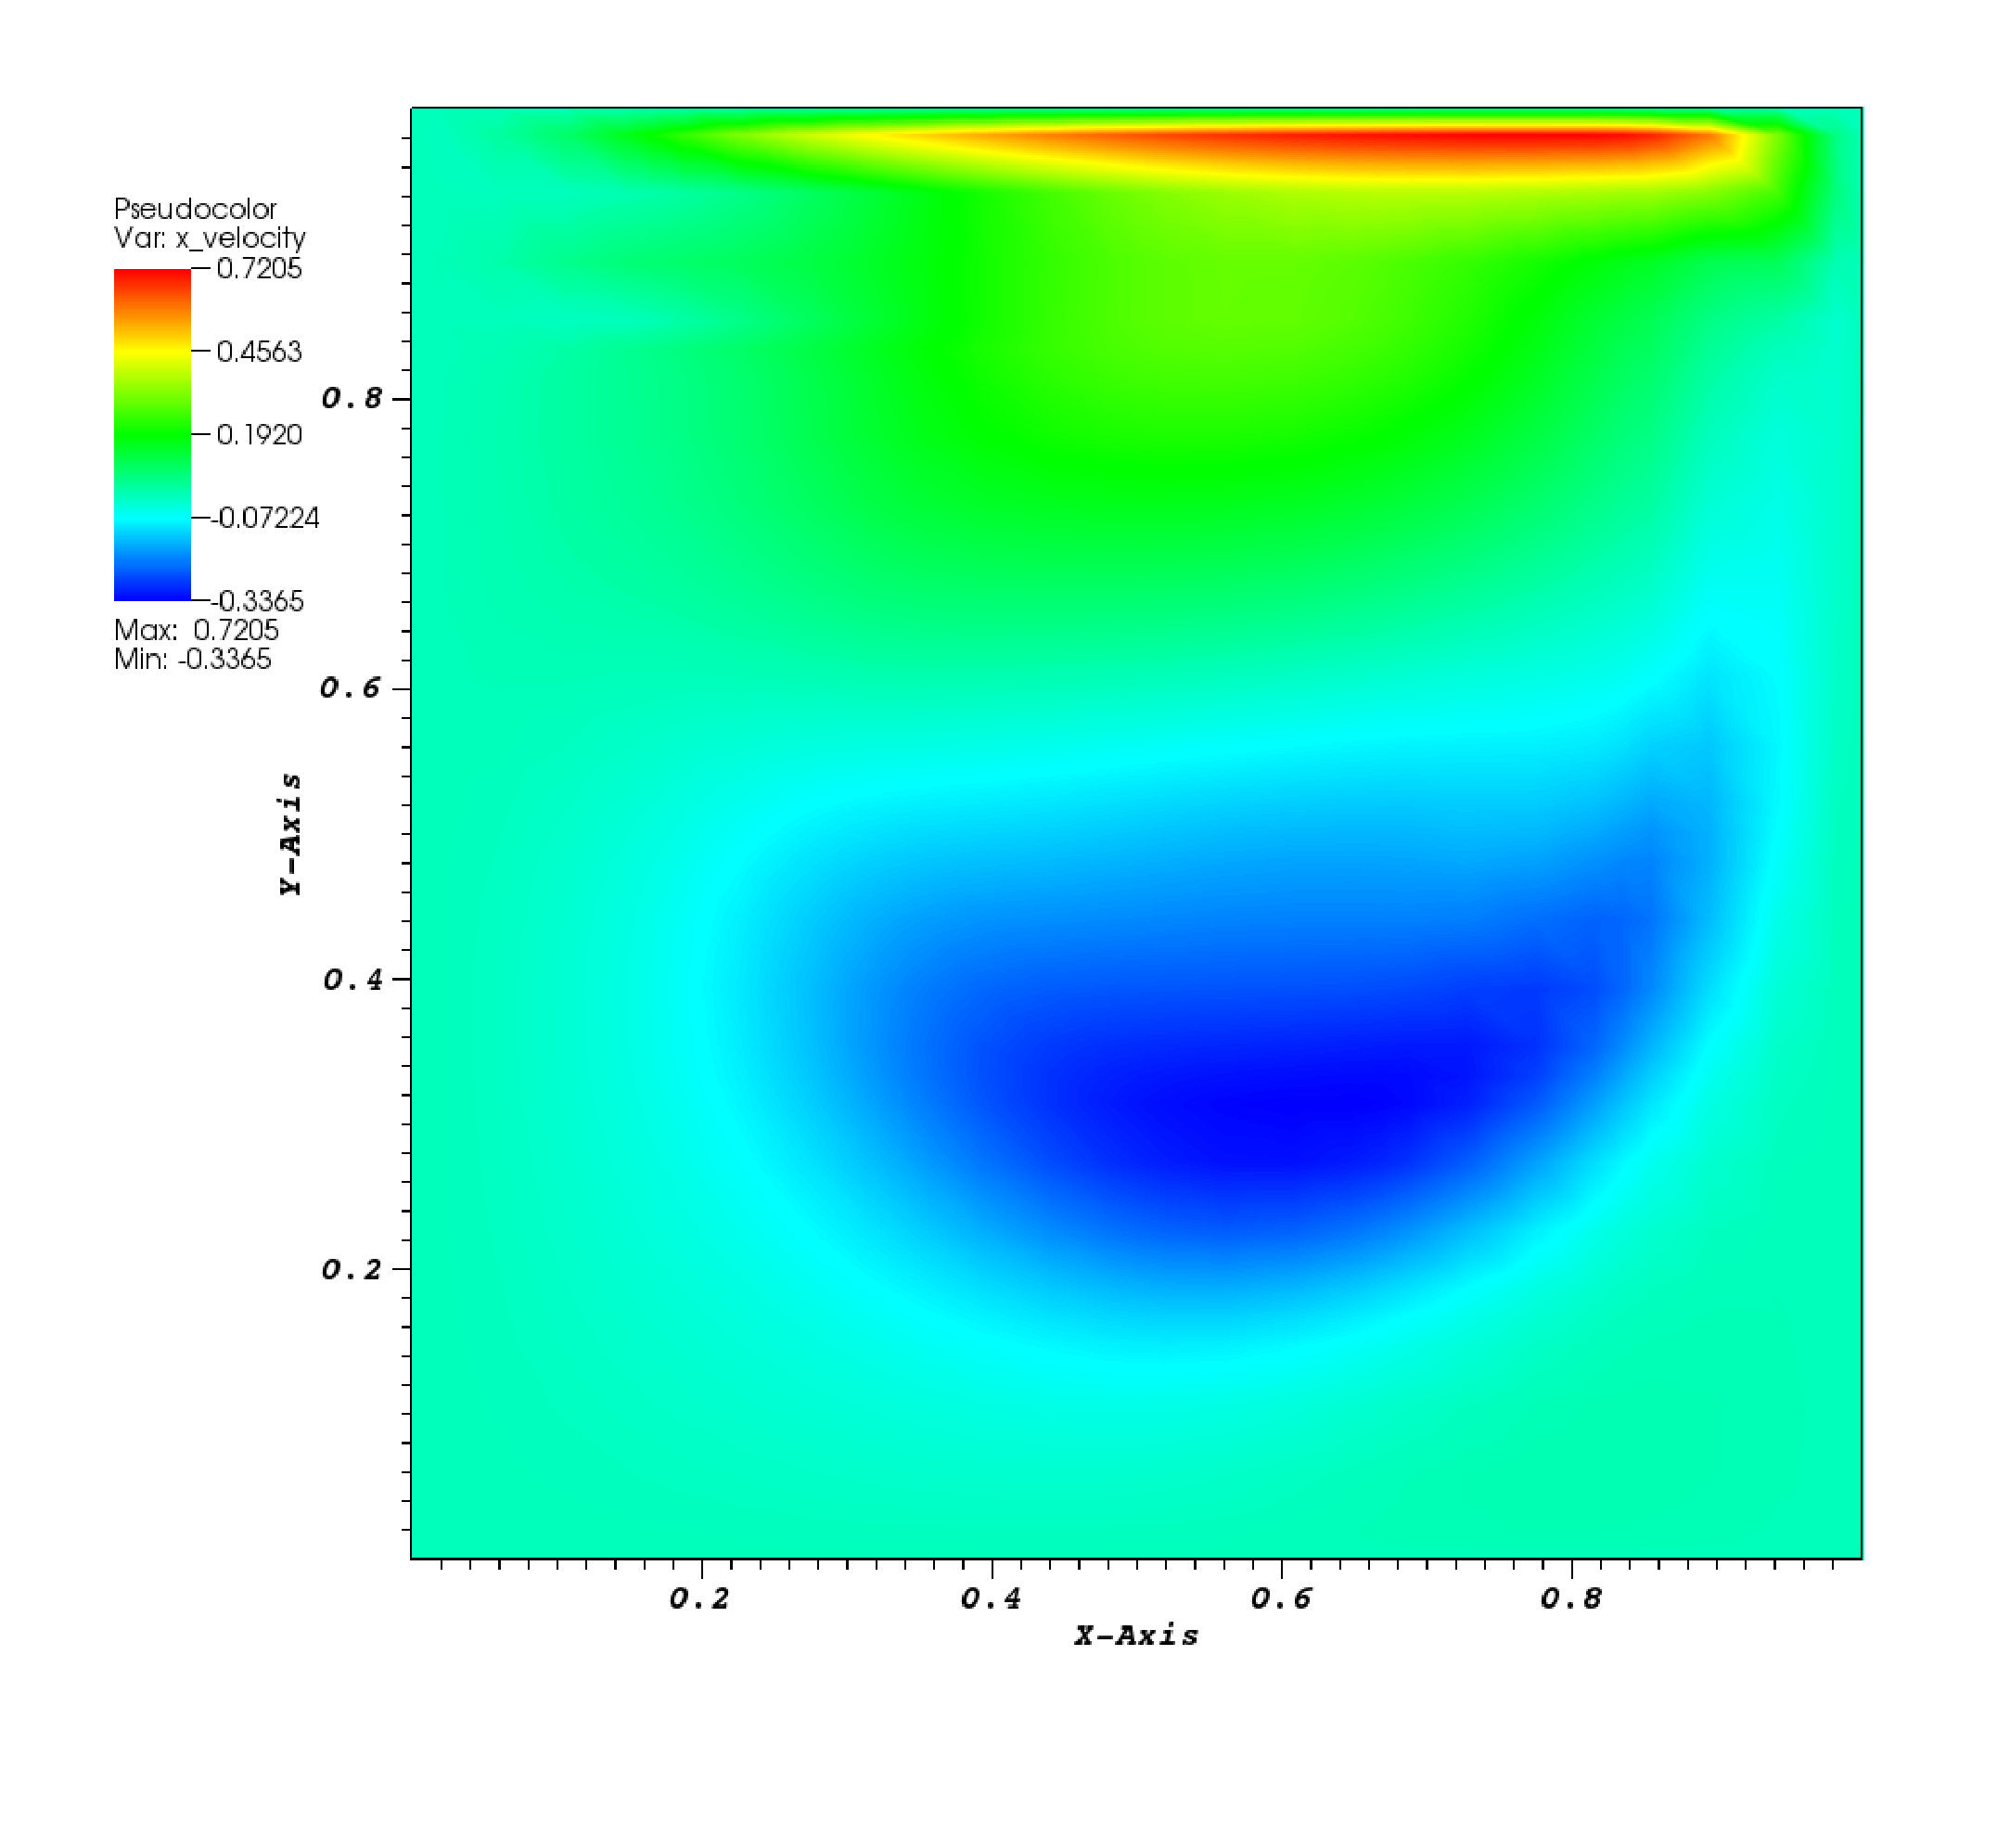
\includegraphics[width=0.45\textwidth]{./figures/grad_adj}}
  \subfigure[Finite difference]{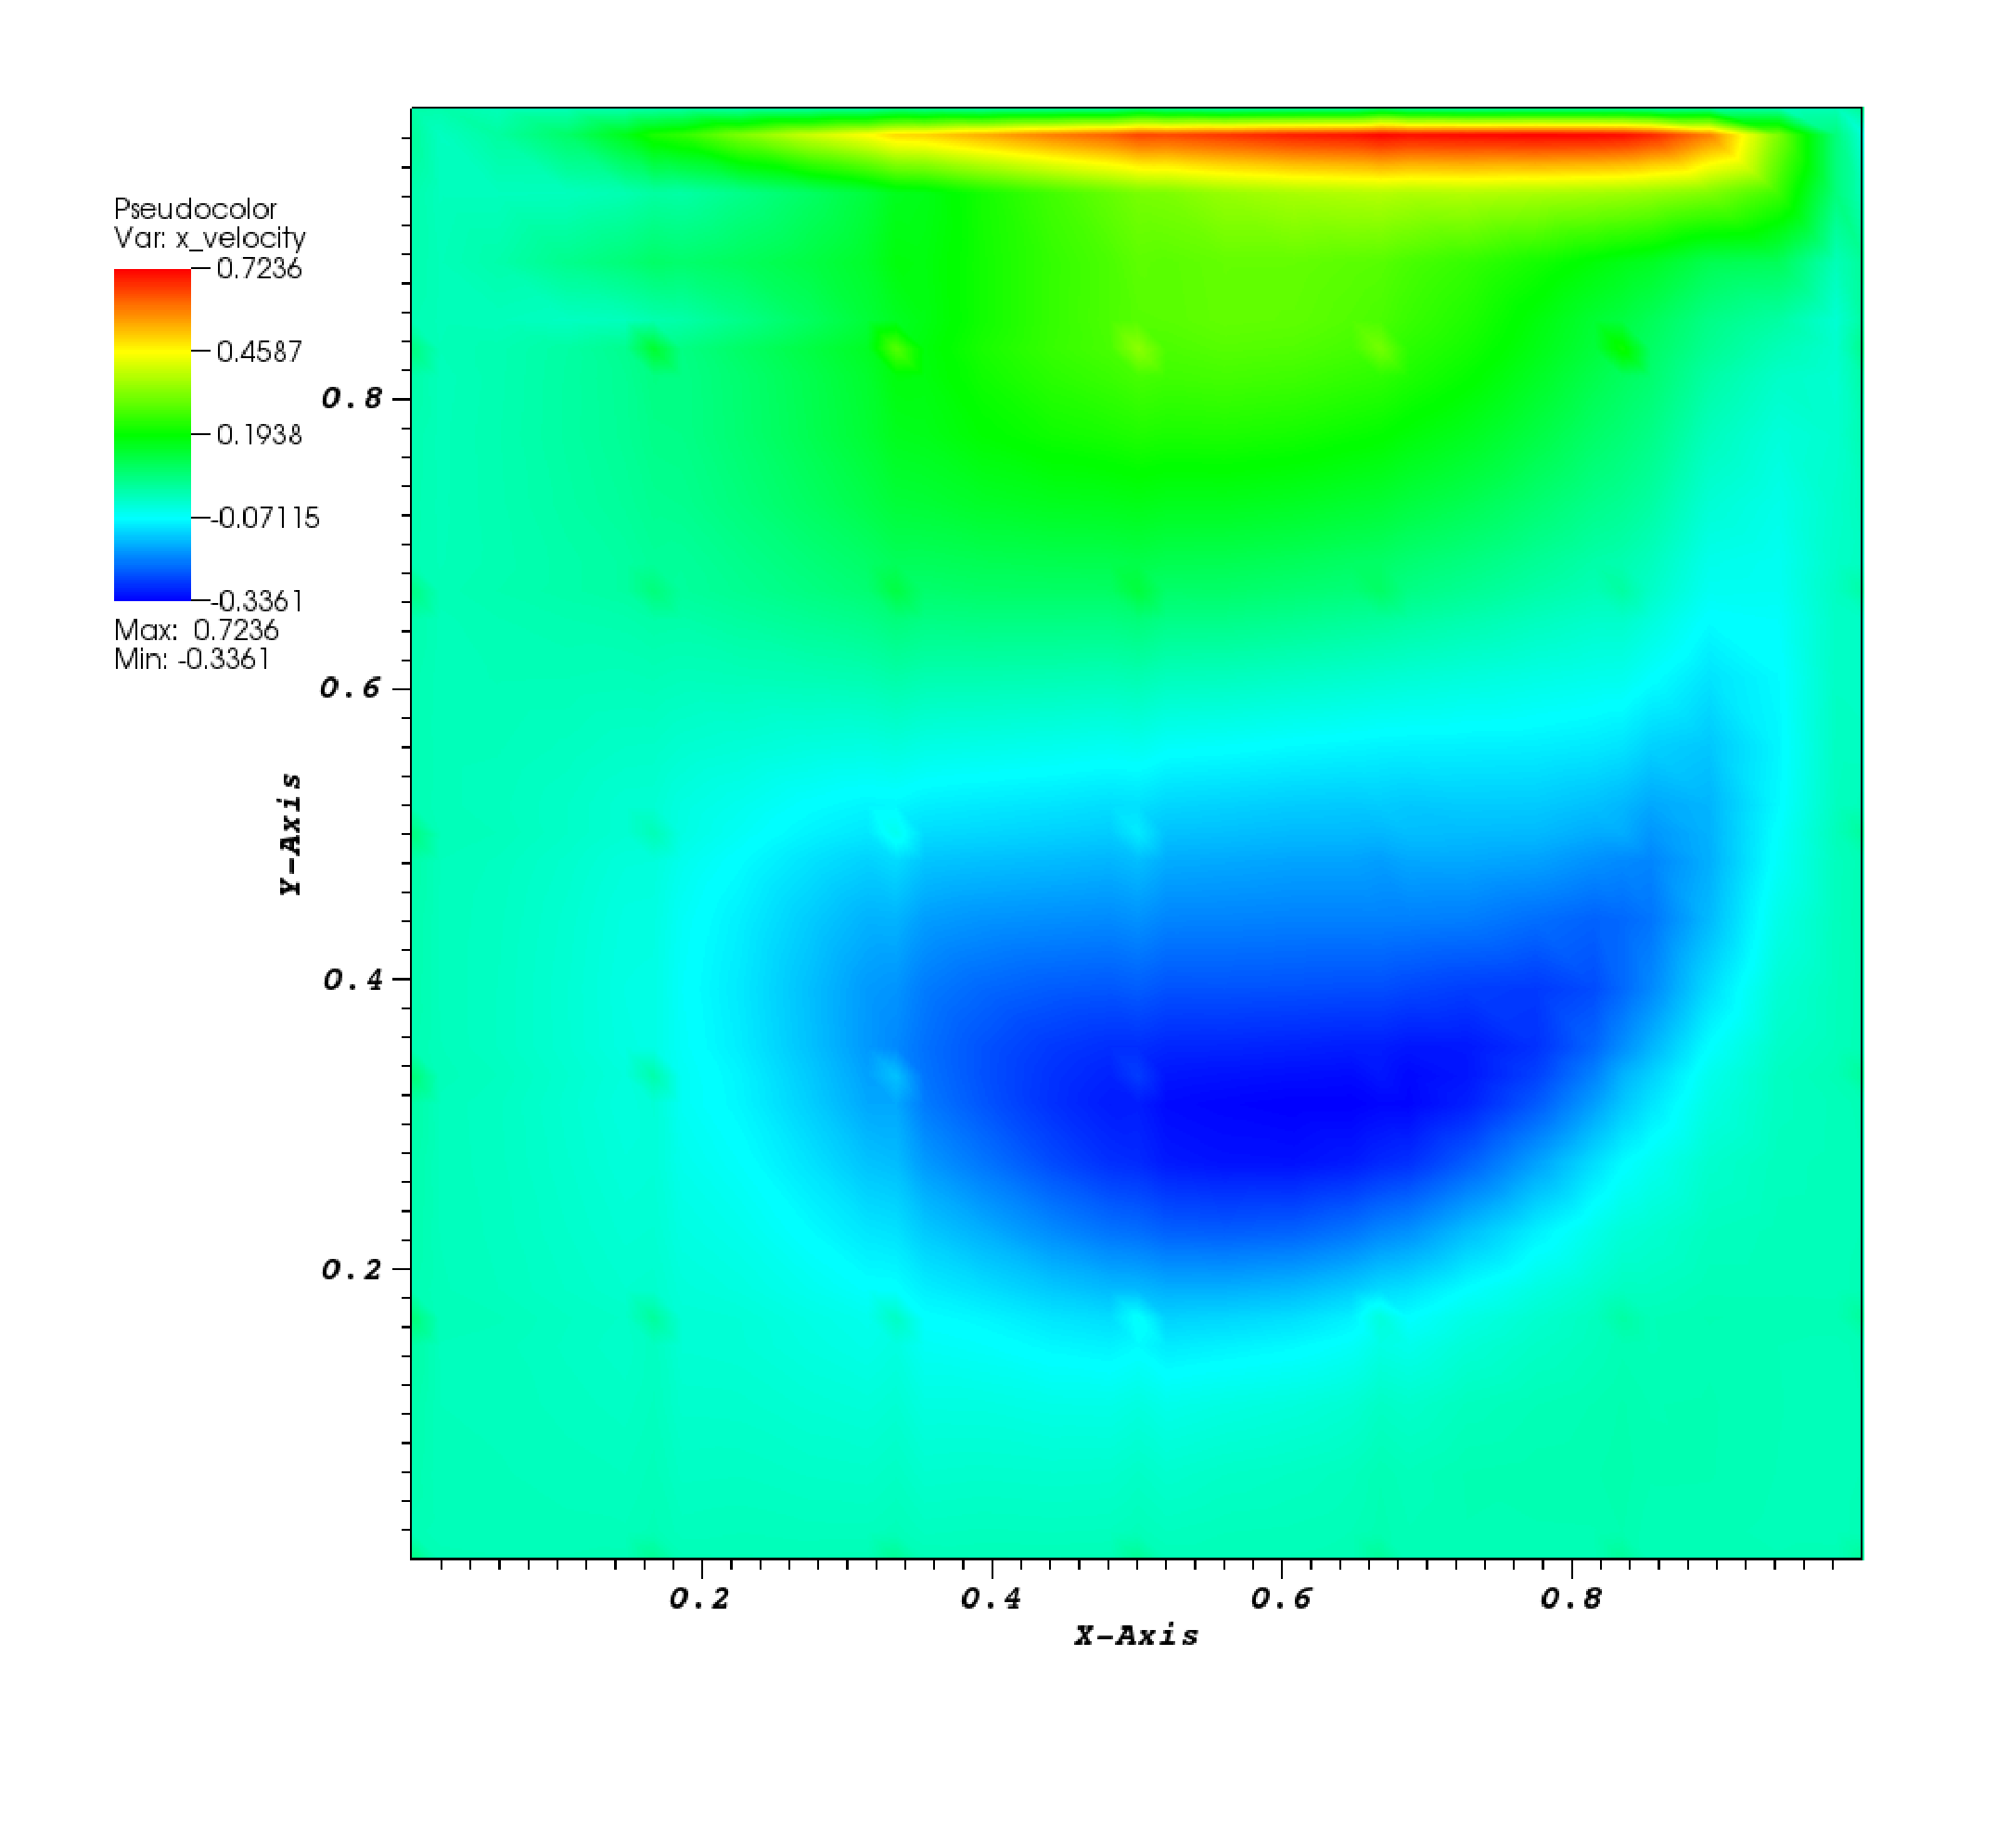
\includegraphics[width=0.45\textwidth]{./figures/grad_fd_rescale}}
  \caption{Validation of the gradient in $x$
  direction computed of the energy $E_k$ at time step $t$ with respect to
  velocity $\mathbf{u}$ at time step $t-1$ via adjoint and finite
  difference in the 2d lid driven cavity.}
  \label{fig:fd}
\end{figure}
\end{frame}

\begin{frame}
  \frametitle{Algorithm on Mira using Nek5000}
  \begin{itemize}
    \item Assuming 50 memory checkpoints (3D $\rightarrow$ 150 vector fields)
    \item Stride q determines performance of revolve and the entire adjoint run
    \item Stride size is between 50 and 3000 depending on {\color{darkgreen}problem
      size}, {\color{blue}time step wall clock time} and {\color{red}bandwidth} 
    \item Bandwidth to archive on Mira is {\color{red}$2GB/s$}, 1 time step of
      Nek is around {\color{blue}$1s$}
    \item Independent of number of nodes!
    \item Example: 10B degrees of freedom $\rightarrow$ {\color{darkgreen}400GB} per checkpoint, stride size:
      {\color{darkgreen}$400$}/{\color{red}$2$}=200/{\color{blue}$1$}=200
  \end{itemize}
  \begin{center}
    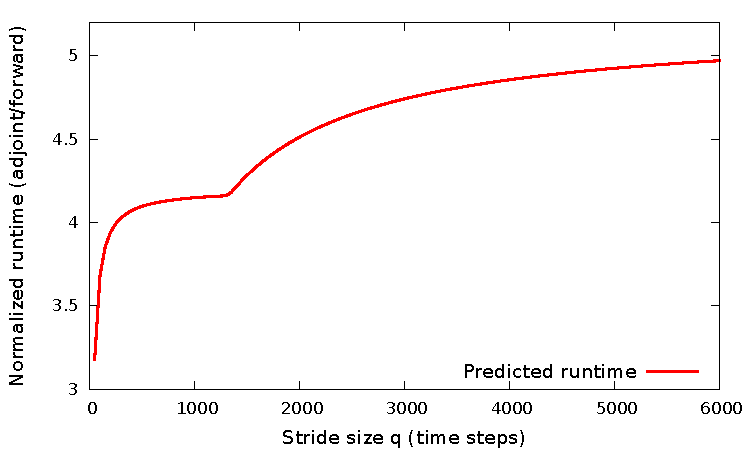
\includegraphics[width=0.6\textwidth]{./figures/revolve_pred}
  \end{center}
\end{frame}


\begin{frame}
  \frametitle{Verification of Performance Model}
  \begin{figure}
    \centering
    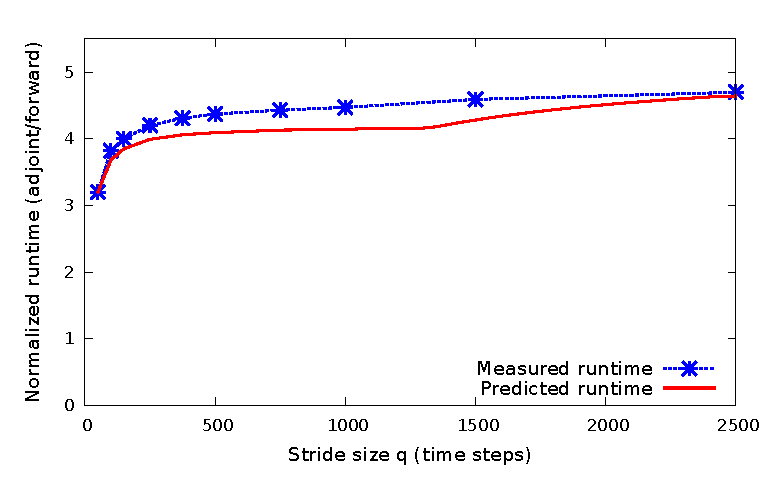
\includegraphics[width=0.8\textwidth]{./figures/revolve}
    %\caption{ The predicted ratio assumes that storing
    %and restoring checkpoints has no cost and one adjoint and primal solve for one
    %time step have the same runtime. The seeming diskontinuity in the
    %predicted time marks the point at $\binom{s+2}{s}=\binom{52}{50}=1300$
    %mentioned in \alert{intro}. This point marks maximum reusage of the checkpoints and
    %thus also maximum memory access, hinting at the largest difference at this
    %point between measured and predicted curve in life experience. 
    %For \lstinline{revolve} 50 checkpoints were used on 8,192 cores (512 nodes) at a problem size of
    %$100,000$ degrees of freedom per core. The disk I/O bandwidth during the forward run
    %determines the stride of time steps that revolve will be applied to. 
    %The predicted runtime was analytically derived and serves as a lower bound.
    %Revolve neglects memory access time.}
    \label{fig:revolve}
  \end{figure}
  \begin{itemize}
    \item 50 checkpoints on 512 nodes (8192 cores), $100000$ DoF per core
    \item Normalized runtime=ratio adjoint/forward runtime
    \item Predicted kink at $\binom{s+2}{s}=\binom{52}{50}=1300$
    \item I/O \alert{bandwidth} determines stride size
    \item Predicted curve ignores memory latency
  \end{itemize}
\end{frame}

\begin{frame}
  \frametitle{Validation: Weak Scaling}
  \begin{figure}
    \centering
    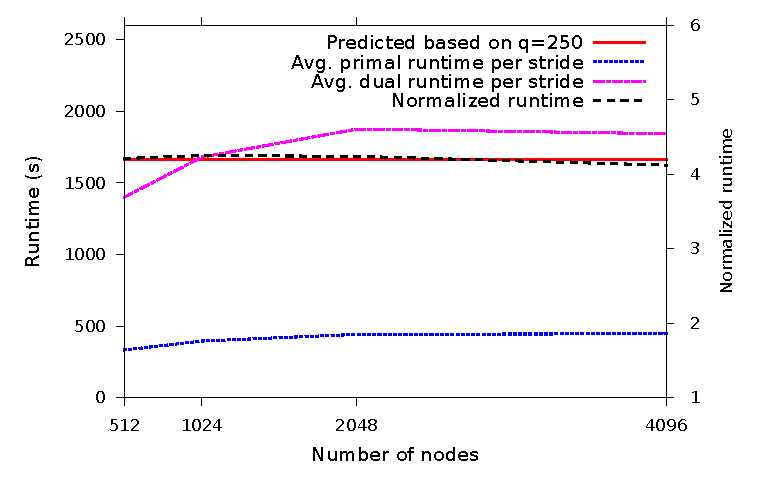
\includegraphics[width=0.8\textwidth]{./figures/strong}
    %\caption{Runs conducted with a stride size of 250 and 50 memory
    %checkpoints per stride. The average runtime of the forward run and adjoint run
    %per stride represent
    %the weak scaling behavior of Nek5000. The normalized runtime stays
    %constant with increasing number of nodes.}
    \label{fig:revolve_strong}
  \end{figure}
  \begin{itemize}
    \item Fixed stride size of $q=250$ and 50 memory checkpoints
    \item Normalized runtime stays constant
    \item This may be an additional requirement/assumption about the underlying
      code
  \end{itemize}
\end{frame}

\begin{frame}
  \frametitle{Final slide\ldots}
 {\bf Summary}
  \begin{itemize}
    \item Asynchronous two-level checkpointing
    \item Recomputation/memory trade-off
    \item Implementing a high latency stack in HPC
    \item Stretch out checkpoints all down the memory hierarchy
    \item Performance model
    \item Interface is hardware dependent
  \end{itemize}
  
  {\bf Open questions/Outlook}
 \begin{itemize}
   \item Generic nonlinear adjoint model for Nek5000
   \item Lossy and lossless compression
   \item Include synchronous disk in checkpointing, PETSc implementation
   \item Noise in I/O to archive
 \end{itemize}
\end{frame}

\begin{frame}
  \begin{center}
    {\Huge \bf Thank you.}
  \end{center}
\end{frame}

\begin{frame}{References}
\bibliographystyle{plainnat}
\bibliography{presentation}
\end{frame}


\begin{frame}
  \frametitle{Stride Sizes at Various Problem Sizes}
\begin{table}
  \centering
  %\begin{tabular}{||x{0.6cm}|x{1.2cm}||c|x{1.2cm}|x{1.2cm}||}
  \begin{tabular}{||c|c||c|c|c||}
    \hline
    \multicolumn{2}{||c||}{\bf Problem Size}&\multicolumn{3}{c||}{\bf Estimations}\\
    \hline
    {\bf DoF} & {\bf Size (GB)} & {\bf Nodes} &{\bf Stride Size
    (ts)} &{\bf Norm. runtime}\\ 
    \hline
    3.2B & 95   & 2048   & 47.5   & 3.3\\ 
    6.5B & 189  & 4096   & 94.5   & 3.7\\
    13B  & 377  & 8192   & 188.5  & 4.0\\
    26B  & 754  & 16384  & 377  & 4.3\\
    52B  & 1507 & 32768  & 753.5  & 4.4\\ 
    52B  & 6028 (multistep) & 32768  & 3014 & 4.6\\
    \hline
  \end{tabular}
  \caption{Estimated stride size for a given problem size with $\approx$ 50000
  degrees of freedom per node and a bandwidth of 2GB/s}
  \label{tab:stride}
\end{table}
\end{frame}


